%%%%%%%%%%%%%%%%%%%%%%%%%%%%%%%%%%%%%%%%%
% Beamer Presentation
% LaTeX Template
% Version 1.0 (10/11/12)
%
% This template has been downloaded from:
% http://www.LaTeXTemplates.com
%
% License:
% CC BY-NC-SA 3.0 (http://creativecommons.org/licenses/by-nc-sa/3.0/)
%
%%%%%%%%%%%%%%%%%%%%%%%%%%%%%%%%%%%%%%%%%

%----------------------------------------------------------------------------------------
%	PACKAGES AND THEMES
%----------------------------------------------------------------------------------------

\documentclass[xcolor=svgnames]{beamer}

\mode<presentation> {

% The Beamer class comes with a number of default slide themes
% which change the colors and layouts of slides. Below this is a list
% of all the themes, uncomment each in turn to see what they look like.

% \usetheme{default}
% \usetheme{AnnArbor}
% \usetheme{Antibes}
%\usetheme{Bergen}
% \usetheme{Berkeley}
% \usetheme{Berlin}
\usetheme{Boadilla}
% \usetheme{CambridgeUS}
% \usetheme{Copenhagen}
% \usetheme{Darmstadt}
% \usetheme{Dresden}
% \usetheme{Frankfurt}
% \usetheme{Goettingen}
% \usetheme{Hannover}
% \usetheme{Ilmenau}
% \usetheme{JuanLesPins}
% \usetheme{Luebeck}
% \usetheme{Madrid}
% \usetheme{Malmoe}
% \usetheme{Marburg}
% \usetheme{Montpellier}
% \usetheme{PaloAlto}
% \usetheme{Pittsburgh}
% \usetheme{Rochester}
% \usetheme{Singapore}
% \usetheme{Szeged}
% \usetheme{Warsaw}

% As well as themes, the Beamer class has a number of color themes
% for any slide theme. Uncomment each of these in turn to see how it
% changes the colors of your current slide theme.

% \usecolortheme{albatross}
% \usecolortheme{beaver}
%\usecolortheme{beetle}
% \usecolortheme{crane}
%  \usecolortheme{dolphin}
% \usecolortheme{dove}
% \usecolortheme{fly}
% \usecolortheme{lily}
% \usecolortheme{orchid}
% \usecolortheme{rose}
% \usecolortheme{seagull}
% \usecolortheme{seahorse}
% \usecolortheme{whale}
% \usecolortheme{wolverine}

% \setbeamertemplate{footline} % To remove the footer line in all slides uncomment this line
%\setbeamertemplate{footline}[page number] % To replace the footer line in all slides with a simple slide count uncomment this line

% \setbeamertemplate{navigation symbols}{} % To remove the navigation symbols from the bottom of all slides uncomment this line
}

\usepackage{graphicx} % Allows including images
\usepackage{booktabs} % Allows the use of \toprule, \midrule and \bottomrule in tables
\usepackage{tikz}
\usepackage{multicol}
\usepackage{wrapfig}
\usepackage{amsmath,amsthm,amssymb}
\usepackage{mathtools}
\usepackage{hyperref}
\DeclarePairedDelimiter\ceil{\lceil}{\rceil}
\DeclarePairedDelimiter\floor{\lfloor}{\rfloor}


\addtobeamertemplate{frametitle}{}{%
\begin{tikzpicture}[remember picture,overlay]
\node[anchor=north east,yshift=2pt] at (current page.north east) {
\includegraphics[height=0.8cm]{iiit-new.png}};
\end{tikzpicture}}

\setbeamercolor{title in head/foot}{bg=OrangeRed, fg=White}
\setbeamercolor{author in head/foot}{bg=RoyalBlue, fg=White}
\setbeamercolor{date in head/foot}{bg=SlateGray, fg=Black}

%----------------------------------------------------------------------------------------
%	TITLE PAGE
%----------------------------------------------------------------------------------------

\title[Discrete Structures]{Discrete Structures} % The short title appears at the bottom of every slide, the full title is only on the title page
\author{IIIT Hyderabad} % Your name
\institute[] % Your institution as it will appear on the bottom of every slide, may be shorthand to save space
{
Monsoon 2020 \\ % Your institution for the title page
\medskip
\textit{Tutorial 7} % Your email address
}
\date{October 7, 2020} % Date, can be changed to a custom date

\begin{document}

\begin{frame}
\titlepage % Print the title page as the first slide
\end{frame}

\begin{frame}
\frametitle{Introduction} % Table of contents slide, comment this block out to remove it
\tableofcontents % Throughout your presentation, if you choose to use \section{} and \subsection{} commands, these will automatically be printed on this slide as an overview of your presentation
\end{frame}

%----------------------------------------------------------------------------------------
%	PRESENTATION SLIDES
%----------------------------------------------------------------------------------------

%------------------------------------------------
\section{Questions}
%------------------------------------------------

%------------------------------------------------
\subsection{Question 0}
%------------------------------------------------
\begin{frame}{Question 0}
    Consider elliptic curve $E_{5}(2,1)$ or in equation form as -
    \begin{align*}
        y^2 &= x^3 + 2x + 1
    \end{align*}
    If $P=(1,3)$ and $Q = (3,2)$ lie on the above curve, find $-2P +     2Q$.
    \\ \textbf{\underline{Sol:}} We calculate 2P first.
        \begin{align*}
            \lambda &= \frac{3\cdot 1 + 2}{6}
                \\  &= 0
                \\ x_R &= 0 - x_P - x_P
                \\ &= -2 = 3
                \\ y_R &= 0(x_P - x_R) - y_P
                \\ &= -3 = 2
        \end{align*}
\end{frame}
\begin{frame}{}
\footnotesize{
    We calculate 2Q next.
        \begin{align*}
            \lambda &= \frac{3\cdot 3 + 2}{4}
                \\  &= 2
                \\ x_R &= 2 - x_Q - x_Q
                \\ &= -4 = 1
                \\ y_R &= 2(x_Q - x_R) - y_Q
                \\ &= 2
        \end{align*}
        We get (3,2) thus, -2P is (3,-2) or (3,3) and 2Q is (1,2). Now we calculate -2P + 2Q.
        \begin{align*}
            \lambda &= \frac{2 - 3}{1 - 3}
                \\    &= 3
                \\ x_R &= 3 - x_{-2P} - x_{2Q}
                \\ &= -1 = 4
                \\ y_R &= 3(x_{-2P} - x_R) - y_{-2P}
                \\ &= -6 = 4
        \end{align*}
        Thus we get (4,4).
    }
\end{frame}

%------------------------------------------------
\subsection{Question 1}
%------------------------------------------------

\begin{frame}{Question 1}
        What are the sets in the partition of the integers arising from congruence modulo 4? \\
        \textbf{\underline{Sol:}} We know the four congruence classes are $[0]_4, [1]_4, [2]_4, [3]_4$, i.e., integers which give remainder $0, 1, 2, 3$ when divided by $4$:\\
        $[0]_4 = \{\dots, -8, -4, 0, 4, 8, \ldots\}$\\
        $[1]_4 = \{\dots, -7, -3, 1, 5, 9, \ldots\}$\\
        $[2]_4 = \{\dots, -6, -2, 2, 6, 10, \ldots\}$\\
        $[3]_4 = \{\dots, -5, -1, 3, 7, 11, \ldots\}$\\
\end{frame}

%------------------------------------------------
\subsection{Question 2}
%------------------------------------------------

\begin{frame}{Question 2}
    Determine which one of these are equivalence and list their equivalence classes (if applicable). Also if it isn't an equivalence relation tell which property does it lack:
    \begin{enumerate}
        \item $\{(a,b) | a \text{ and } b \text{ are the same age}\}$ \\
        \textbf{\underline{Sol:}} Equivalence. $[a]_R = \{b \in A | b \text{ has the same age as } a\}$
        \item $\{(a, b) | a \text{ and } b \text{ have the same parent}\}$ \\
        \textbf{\underline{Sol:}} Equivalence. $[a]_R = \{b \in A | b \text{ has the same parent as } a\}$
        \item $\{(a, b) | a \text{ and } b \text{ have met}\}$ \\ 
        \textbf{\underline{Sol:}} Not transitive. 
        \item $\{(a, b) | a \text{ and } b \text{ speak a common language}\}$ \\
        \textbf{\underline{Sol:}} Not transitive
    \end{enumerate}
\end{frame}

%------------------------------------------------
\subsection{Question 3}
%------------------------------------------------

\begin{frame}{Question 3}
    \textbf{3.1} Which of the following are partitions of $S = \{1, 2, 3, 4, 5, 6\}$:
    \begin{enumerate}
        \item $\{1, 2\}, \{2, 3, 4\}, \{4, 5, 6\}$
        \\\textbf{\underline{Sol:}} False. $\{1, 2\} \cap \{2,3,4\} \neq \phi$
        \item $\{1\}, \{2, 3, 6\}, \{5\}, \{4\}$
        \\\textbf{\underline{Sol;}} True. $\bigcup_{i=1}^4 A_i = S$ and $A_i \cap A_j = \phi\  \forall i, j$
    \end{enumerate}
    \textbf{3.2} Which of the following are partitions of the set of real numbers:
    \begin{enumerate}
        \item Set of intervals $[k, k+1], k =\ldots -2, -1, 0, 1, \ldots$
        \\\textbf{\underline{Sol:}} False. $[1, 2] \cap [2, 3] \neq \phi$, i.e. $[k, k+1] \cap [k+1, k+2] = \{k\}\  \forall k$
        \item Set of intervals $(k, k+1), k =\ldots -2, -1, 0, 1, \ldots$
        \\\textbf{\underline{Sol:}} False. $\bigcup_{k \in \mathbb{Z}} (k, k+1) \neq \mathbb{R}$. Actually it is the set $\mathbb{R} - \mathbb{Z}$
        \item The sets $\{x + n | n \in \mathbb{Z}\}$ for all $x \in [0, 1)$
        \\\textbf{\underline{Sol:}} True. $x$ covers the real numbers between any $2$ integers, and $n$ expands it to all integers. Also $\{x + n_1\} \cap \{x + n_2\} = \phi \ \forall n_1, n_2 \in \mathbb{Z}$
    \end{enumerate}
\end{frame}

\begin{frame}{Question 3}
    \textbf{3.3} Verify whether it is a partitions of the set $\mathbb{Z}\times\mathbb{Z}$ of ordered pair of integers: \\
    The set of pairs $(x, y)$, where $3 \mid x$ and $3 \mid y$; the set of pairs $(x,y)$, where $3 \mid x$ and $3 \nmid y$; the set of pairs $(x, y)$ where $3 \nmid x$ and $3 \mid y$; the set of pairs $(x,y)$ where $3 \nmid x$ and $3 \nmid y$
    \\\textbf{\underline{Sol:}} First partition: $(x,y) = (3p, 3q)\ p, q \in \mathbb{Z}$; Second partition: $(x, y) = (3p, 3q + r)\ p, q \in \mathbb{Z}, r = 1, 2$; Third partition: $(x, y) = (3p + r, 3q)\ p, q \in \mathbb{Z}, r= 1, 2$; Fourth partition: $(x, y) = (3p + r_1, 3q + r_2)\ p, q \in \mathbb{Z}, r_1,r_2 = 1, 2$. \\ 
    Now, $P_i \cap P_j = \phi\ \forall i, j$ because $3m \neq 3n + r, r=1,2\  \forall m, n \in Z$ (now either $x$ or $y$ or both won't be satisfied in the intersect condition).\\
    To show that the union of the partitions leads to $\mathbb{Z}\times\mathbb{Z}$ can be done in many ways. Consider constructing base examples and show that all possible integers can be represented by adding $3$. Another way may be to pair up the partitions as ones where $x = y$ and $x \neq y$ and show that they represent that for all $x, y \in \mathbb{Z}$ and that their union gives all cases of $\mathbb{Z}\times\mathbb{Z}$
\end{frame}

%------------------------------------------------
\subsection{Question 4}
%------------------------------------------------

\begin{frame}{Question 4}
    \textbf{4.1} Let $R$ be the relation on the set of all people who have visited a particular Web page such that $xRy$ if and only if person $x$ and person $y$ have followed the same set of links starting at this Web page (going from Web page to Web page until they stop using the Web). Find out the properties of the relation $R$. \\ 
    \vspace{4mm}
    \textbf{4.2 a} Let $n$ be a positive integer. Show that the relation $R$ on the set of all polynomials with real-valued coefficients of all pairs $(f, g)$ such that $f^{(n)}(x) = g^{(n)}(x)$ is an equivalence relation. (Here $f^{(n)}(x)$ is the $n$th derivative of $f(x)$) \\ 
    \textbf{4.2 b} Which functions are in the same equivalence class as the function $f(x) = x^4$, where $n = 3$?
\end{frame}

\begin{frame}{Question 4 Solutions}
    \textbf{4.1 \underline{Sol:}} Given, $A$ = Set of all people who have visited a particular Web page\\
    \textbf{Reflexive Let $x \in A$}\\
    Since $x$ always follows the same set of links like itself. Thus $(x,x) \in R$, Thus $R$ is reflexive.\\
    \textbf{Symmetric} Let $(x, y) \in R$.\\
    This means that $x$ and $y$ follows the same link, then $y$ and $x$ follows the same links. Thus $(y, x) \in R$. Thus $R$ is symmetric.\\
    \textbf{Transitive} Let $(x, y) \in R$ and $(y, z) \in R$ \\
    This means that $x$ and $y$ followed the same link, and $y$ and $z$ followed the same link. Thus $x$ and $z$ followed the same links. Thus $(x, z) \in R$. Thus $R$ is transitive \\
    Thus $R$ is an equivalence relation.
\end{frame}

\begin{frame}{Question 4 Solutions}
    \textbf{4.2 a \underline{Sol:}} Given, $A$ = All polynomial functions with real-valued coefficients \\
    \textbf{Reflexive} Let $f \in A$\\
    Since $f^{(n)}(x) = f^{(n)}(x)$ for all $x \in R$. Thus $(f, f) \in R$. Thus $R$ is reflexive.\\
    \textbf{Symmetric} Let $(f, g) \in R$. This means $f^{(n)}(x) = g^{(n)}(x)$, By symmetry of the equality, we get $g^{*n)}(x) = f^{(n)}(x)$ which implies $(g, f) \in R$. Thus $R$ is symmetric \\
    \textbf{Transitive} Let $(f,g) \in R$ and $(g, h) \in R$. Then $f^{(n)}(x) = g^{(n)}(x) = h^{(n)}$. Thus $(f, h) in R$, Thus $R$ is transitive. \\
    Therefore $R$ is an equivalence relation. \\
    \vspace{4mm}
    \textbf{4.2 b \underline{Sol:}} Given $f(x) = x^4$, then $f^{(2)}(x) = 12x^2$. Now for any $g(x)$ we have $g^{(2)}(x) = 12x^2$. Thus $g(x) = x^4 + ax + b$ (by integrating). Thus: 
    \[
        [f]_R = \{g \in A | g^{(2)} = 12x^2\} = \{g \in A | g(x) = x^4 + ax + b\}
    \]

\end{frame}

%------------------------------------------------
\subsection{Question 5}
%------------------------------------------------

\begin{frame}{*Question 5}
    Each bead on a bracelet with three beads is either red, white or blue:
    \begin{figure}
        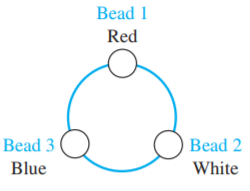
\includegraphics[width=3cm]{dstut7q5.png}
        \label{fig:my_label}
    \end{figure}
    Define the relation $R$ between bracelets as: $(B_1, B_2)$ where $B_1$ and $B_2$ are bracelets, belongs to $R$ if and only if $B_2$ can be obtained from $B_1$ by rotating it or rotating it and then reflecting it. 
    \begin{itemize}
        \item Show that $R$ is an equivalence relation
        \item What are the equivalence classes for $R$
    \end{itemize}
\end{frame}

\end{document} 